\chapter{Brine-Water heat pump Prototype (BWP)}
\label{chap:bwp}
\resetallacronyms

\begin{shaded}
  This chapter presents the \BWP{} designed to demonstrate the
  statement detailed in \cref{chap:methodo}. It presents the prototype
  specifications and design, its results, and the encountered issues.
\end{shaded}

\section{Design of the BWP}
\label{sec:bwp-design}

\subsection{Specifications}
\label{sec:bwp-specs}

\begin{description}
\item[Modularity with the components] The \BWP{} components can be
  changed and many different possibilities can be tested.
\item[Modularity with the thermodynamics cycles and circuits] The
  \BWP{} can test different single and twin-stage heat pump cycles,
  and tolerate modifications of the motor cooling and gas bearings
  aeration circuits.
\item[Liquid refrigerant location monitoring] The \BWP{} is expected
  to allow the tracking of the liquid refrigerant location within the
  cycle. The amount of refrigerant in the heat exchangers and in the
  economizer needs to be known.
\end{description}

Those 3 guidelines led to the following design choices:

\begin{description}
\item[Many assemblies, as few brazings as possible] Ideally, the whole
  setup would have been designed with fittings and assemblies, in
  order to keep as few brazings as possible, but it would have
  exceeded the budget allowed to the manufacturing of the
  prototype. As a compromise, the setup was built with brazed
  components, connected to assembly fittings at their interfaces. The
  system was built around modules which could be relocated or
  connected differently, using flexible or straight pipes, and
  fittings.
\item[Flexible pipes to connect the weighted elements] In order to
  weight the heat exchangers and the economizer properly, those
  components have been hang up to load cells, and connected to the
  main circuits using flexible pipes. This configuration can be
  observed in \cref{fig:bwp-topology}. Those flexible pipes were quite
  rigid, which implied big curvature radius, if they had to be used
  curved.
\item[Inline components with selection of the active component]
  Different types of inline components, such as the expansion valves,
  could be mounted together in parallel in the experimental setup and
  could be operated, alone, or together with the other components of
  the line. This possibility allows to test during the same experiment
  different technologies of valves and active components, in order to
  observe the dynamic response of the cycle\footnotep{An example of a
    test section of expansion devices mounted in parallel can be seen
    in \cpref{sec:bwp-exp-devices}.}. As radial compression units have
  continuous dynamic behavior, changing the dynamics of the valves
  response with different technologies\footnotep{Modulating
    refrigerant valves equipped with a magnetic actuator have a
    response time shorter than stepper-motor valves, but are more
    expensive, for instance. The later valves also have a continuous
    setting behavior while pulse width modulation electric expansion
    valves have a discreet setting behavior. Thermostatic expansion
    valves are cheap but can not be set interactively for the needs of
    the cycle control. Those different technologies have different
    dynamic responses which can have an influence on the dynamic
    behavior of the whole prototype, as the compression unit is a
    dynamic compressor.} can be interesting to develop control
  strategies for the prototypes.
\end{description}

\subsection{Description}
\label{sec:bwp-description}

The \BWP{} is designed to be modular and allows to test different heat
pump layouts. Indeed, each component test section is connected to
other components using fastened fittings and flexible pipes. The
components can be moved and spatially rearranged in the housing. Their
order can also be modified. The experimental setup has been designed to
test single and twin-stage heat pump cycles. The setup is equipped
with load cells to measure the weight of the elements which are
subject to variations of their overall refrigerant vapor
quality. Those weighted components are the condenser, the evaporator,
and the economizer. The weight of the elements was intended to be used
to track the location of the liquid charge in the installation and
would have allowed to compare the observed liquid location behavior
with the predicted behavior using a model of the heat pump integrating
nowadays modeling techniques such as components dynamic modeling and
other techniques listed by \citet{Ding-2007a} in 2007. The model in
question would have been based on moving boundaries heat exchanger
modeling, such as the one implemented by \citet{Bell-Lemort-2015a},
and on mass and energy balance equations. The inline components, such
as the expansion valves, can be mounted in parallel in order to be
tested sequentially or together during the same experiment. Before the
experiment presented in this chapter, the \BWP{} had been modified in
order to get a new bypass circuit which was likely to solve the issues
encountered with the \AWP{} and detailed in
\cref{sec:awp-P-balance}. As explained in \cref{sec:bwp-cp-unit}, the
compression unit crashed soon after the beginning of the experiment
because of an assembly issue in the compression unit. Before the crash
of the unit, a small B8.0/W11.0 \OP{} was being stabilized, with the
compressors being connected in series, bypassed with the new bypass
system. This experiment is interesting as it confirms that the new
bypass circuit, described in \cref{sec:bwp-bypass-system}, is
functional and could consequently maybe solve the issue described in
\cpref{sec:awp-P-balance}. It also shows a thermal behavior of the
compression unit very different of the one observed in the \AWP{}.

\begin{figure}
  \centering
  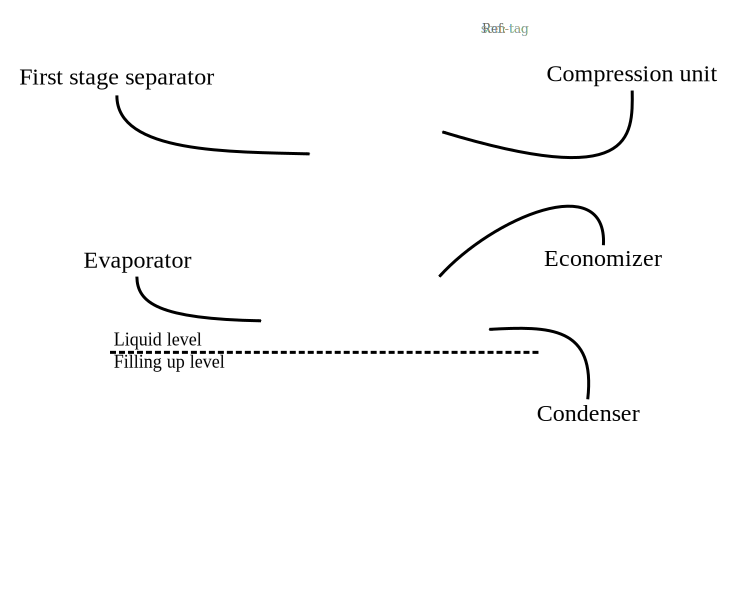
\includegraphics[height=10cm]{bwp-topology}
  \caption{BWP topology, after the first set of heavy modifications
    mentioned in \cref{sec:bwp-redesign-1}.}
  \label{fig:bwp-topology}
\end{figure}

\begin{figure}
  \centering
  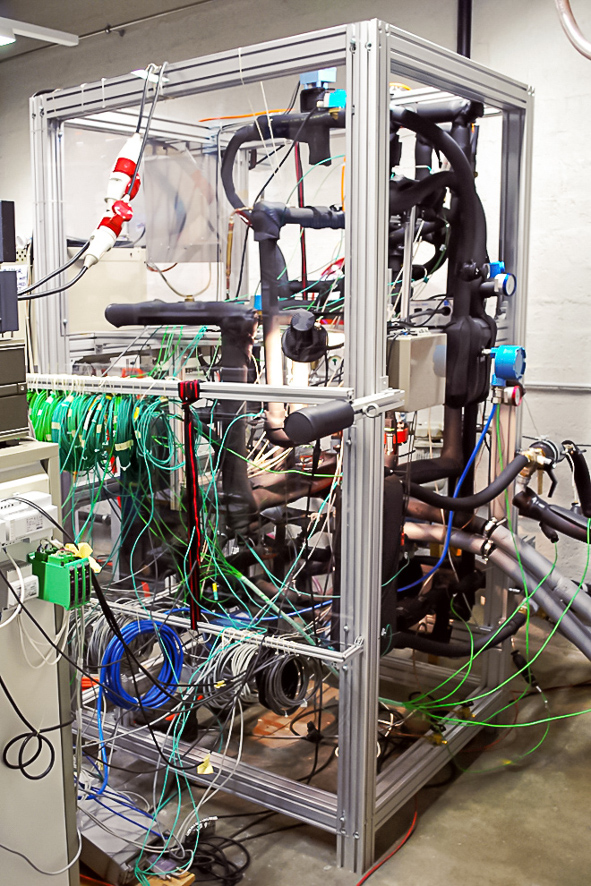
\includegraphics[height=10cm]{20130924T174303-3832-mod}
  \caption{View of the experimental setup in the laboratory.}
  \label{fig:bwp_main_view}
\end{figure}

\begin{figure}
  \centering
  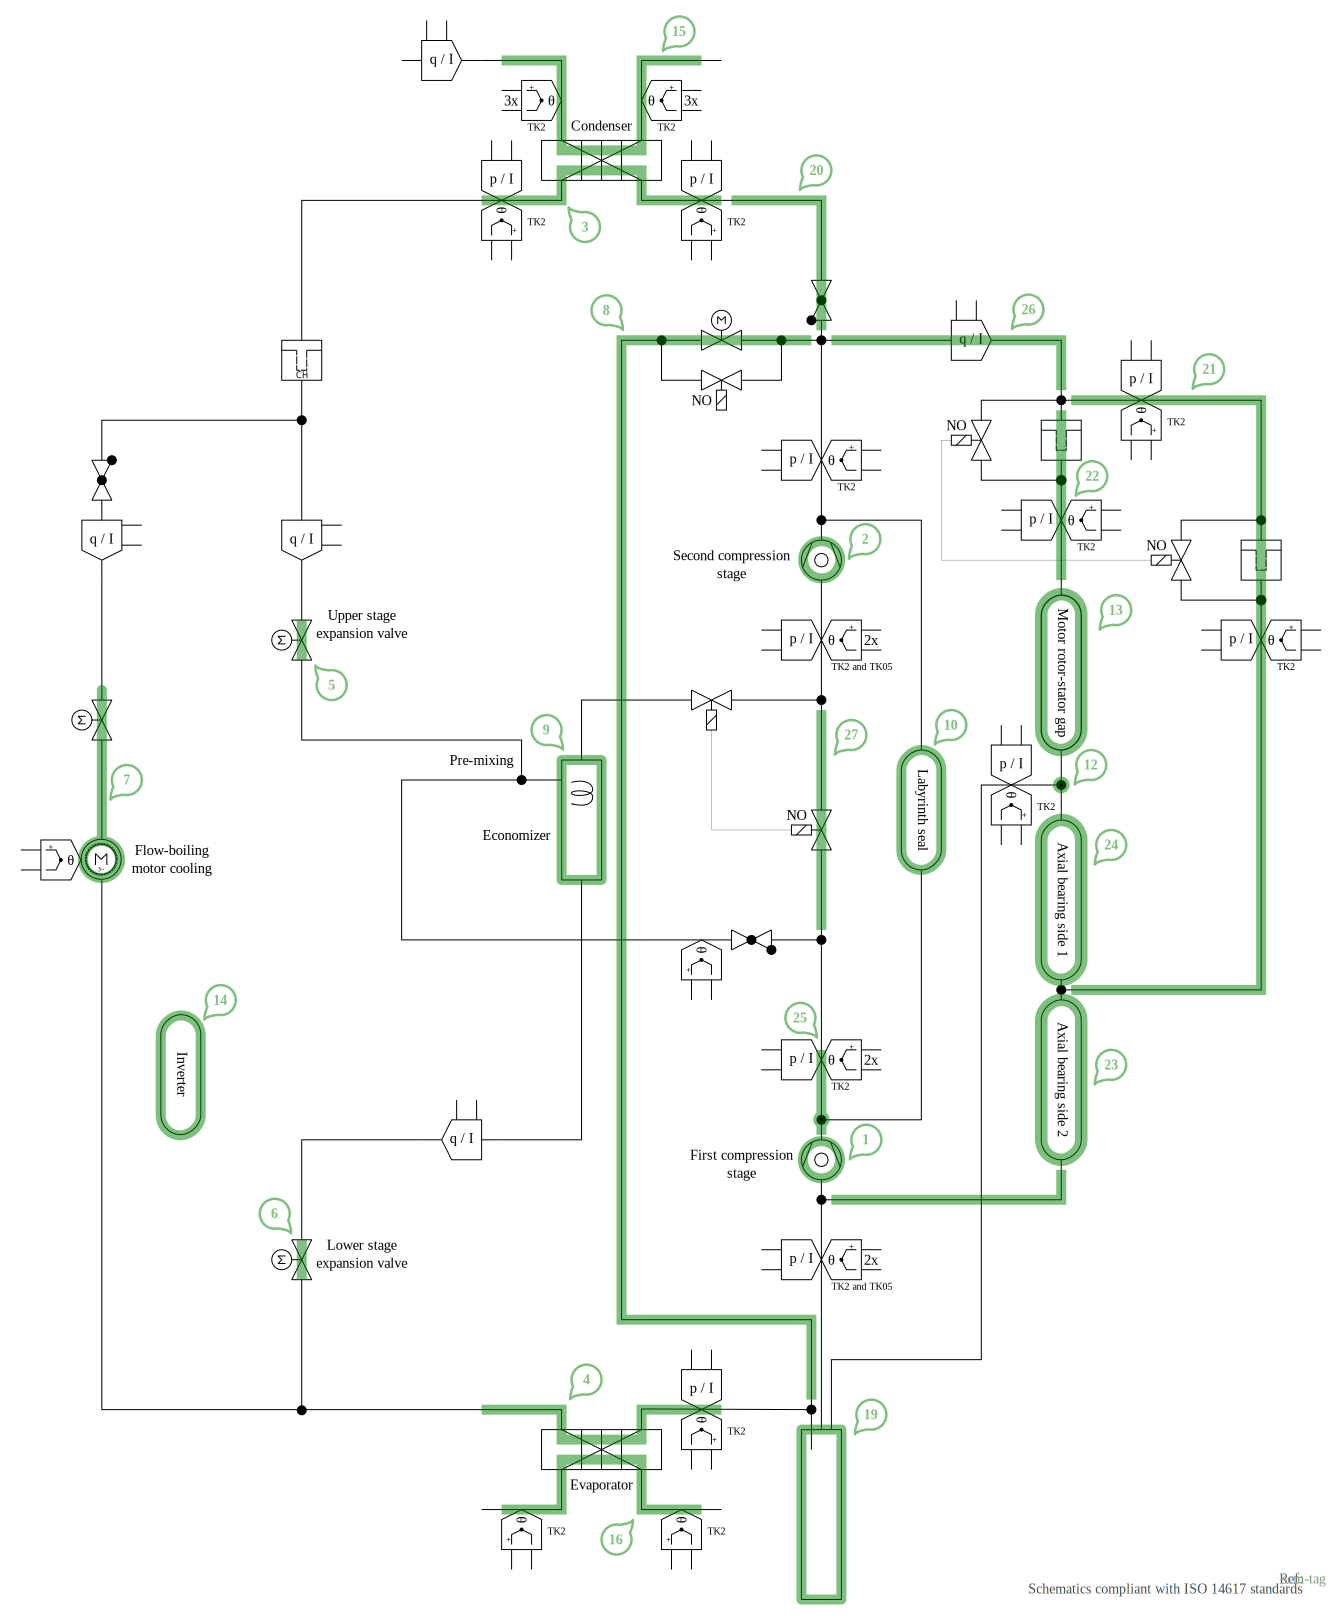
\includegraphics[width=1.0\textwidth]{bwp-layout-maillefer}
  \caption[Layout of the Brine-Water heat pump test-rig]
  {Layout of the Brine-Water heat pump test-rig.}
  \label{fig:bwp-layout}
\end{figure}

The \BWP{} has been designed vertically for liquid management
reasons. Indeed, when the heat pump is stopped:

\begin{itemize}
\item Liquid refrigerant tends to condensate at the evaporator, which
  is the coolest location in the heat pump cycle. Consequently, if no
  insulation valve stops this phenomenon, the evaporator tends to fill
  up with liquid when the installation is stopped.
\item Pumping down the evaporator using radial compression units is a
  difficult operation, as a pump down of the evaporator requires to
  decrease its pressure level, and consequently to support a pressure
  ratio at the first compression stage, which implies to have a flow
  there, but there can be enough flow, as the expansion valve is not
  loaded with liquid refrigerant. \Cref{sec:pump-down-ev} presents the
  issue relative to the pump down of the evaporator.
\end{itemize}

\section{BWP components}
\label{sec:bwp-main-components}

This section gives details about of the main components in order to
make the understanding of the
\crefrange{sec:bwp-model}{sec:bwp-issues} easier. Further details
about the components and the topology of the circuits are given in
\cpref{chap:bwp-components}.

\subsection{Compression unit}
\label{sec:bwp-cp-unit}

The compression unit mounted in the \BWP{} for the experiment which
has been used to generate the data presented in \cref{sec:bwp-perfs}
was the \textit{cp101} unit, from the \textit{evo4} design
family\footnotep{Details about the previous design families are given
  in \cpref{sec:bwp-history}.}. This compression unit has been mounted
in the \BWP{} following the piping layout detailed in
\cref{fig:cp101-struct-bwp}. The compression unit mounted in the
circuits can be seen in \cref{fig:bwp-cp101-mounted}. This piping
layout is very different from the one used with \textit{cp105} in the
\AWP{}. Indeed, the unit \textit{cp101} has been plugged in the heat
pump circuits with the proper inlets and outlets
connections. Unfortunately, due to an assembly issue, the unit crashed
soon after the start of the experiment. After dismantling and
investigation at the industrial partner facility, it appeared that the
unit would have broken in any case due to the mounting defect and the
experiment itself is not responsible for the crash.

\begin{figure}
  \centering
  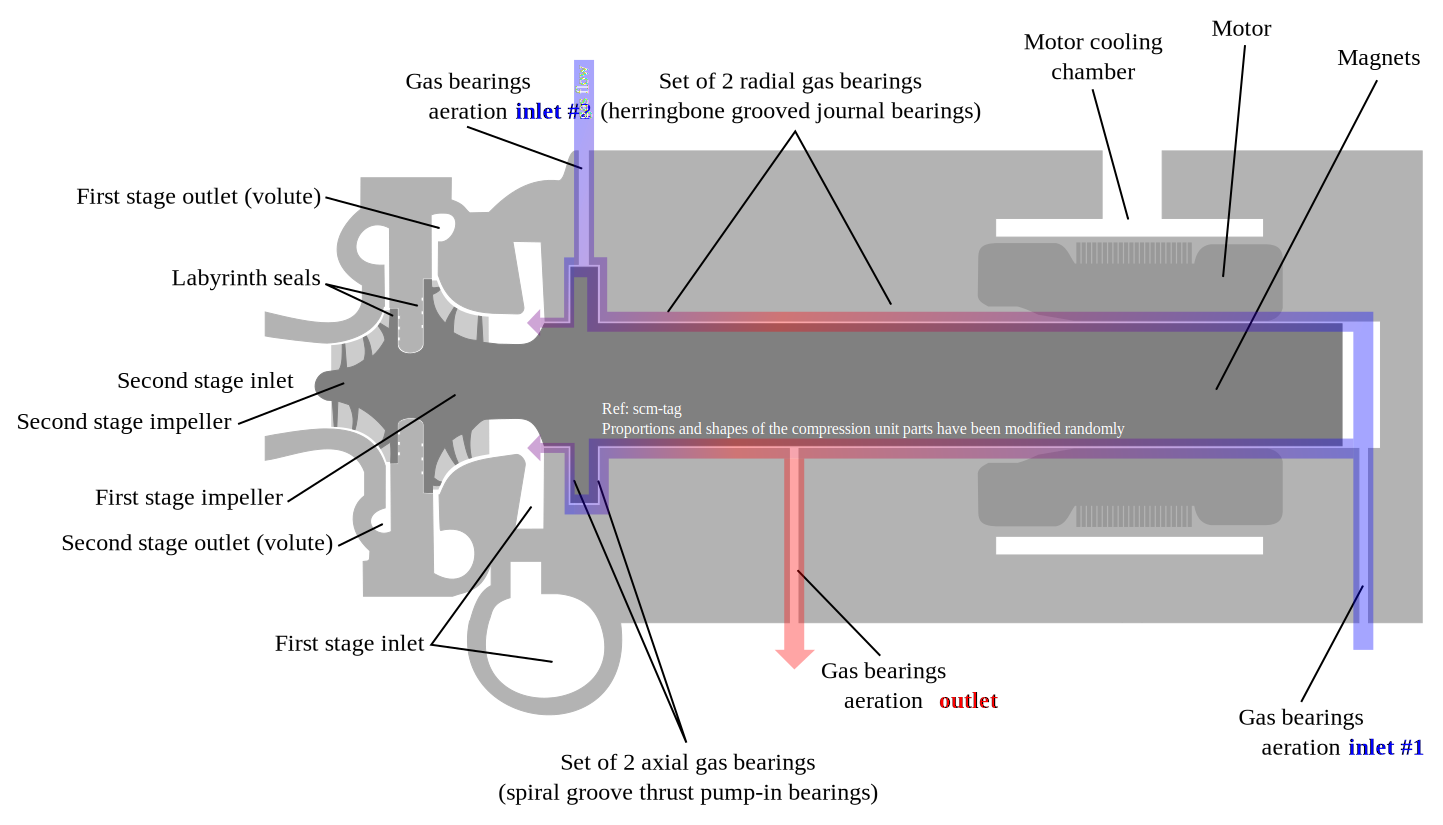
\includegraphics[width=\linewidth]{cp101-wheel-details-bwp}
  \caption[Structure of the compressor unit with the BWP gas bearings
  aeration circuit I/O layout]{Structure of the twin-stage compressor
    unit with the BWP gas bearings aeration circuit I/O layout}
  \label{fig:cp101-struct-bwp}
\end{figure}

\begin{figure}
  \centering
  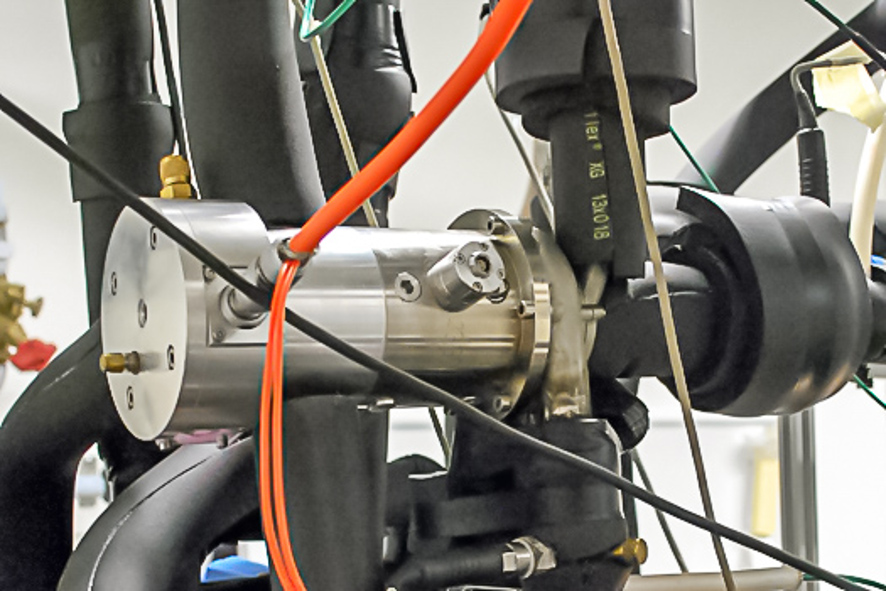
\includegraphics[width=15cm]{20130924T174605-3852-mod}
  \caption{Compression unit \textit{cp101}, mounted in the BWP}
  \label{fig:bwp-cp101-mounted}
\end{figure}

\subsection{Bypass system}
\label{sec:bwp-bypass-system}

The bypass circuit connects the outlet the second compression stage to
the first stage separator (component \#8\footnotep{Components
  numbering is detailed in \cpref{fig:bwp-layout} and
  \cpref{fig:bwp-maillefer-break-model}}). When the bypass circuit is
used, the solenoid valve in component \#27 is opened and no gas from
the vapor line flows into the economizer (component \#9). The
economizer is consequently, in bypass-mode, a simple tank located
after the second-stage expansion valve, ensuring that the first stage
expansion valve is filled up with liquid. In that mode, the economizer
as only one inlet and one outlet\footnotep{In the \AWP{}, the
  economizer has 2 inlets and 2 outlets in every modes.}. In the
\AWP{}, each compression stage has its own bypass-mode and can be
bypassed separately. In the \BWP{}, in bypass-mode, the two
compression stages are in series. The two compression stages have the
same mass flow rate and the intermediate pressure is kept at the
economizer pressure using the second expansion valve
only\footnotep{See issues in \cpref{sec:awp-issue-control}, and
  \cref{sec:bwp-bypass-mode-Pint-issue}, for details about keeping the
  intermediate pressure at a chosen value.}, as the first expansion
valve is dedicated to the setting of the superheat at the outlet of
the evaporator. \Cref{fig:bypass-schematics} shows the complexity of
the configuration of the flows when being in bypass-mode, for the
\AWP{} (\cref{fig:awp-bypass-simple-layout}) and \BWP{}
(\cref{fig:bwp-bypass-simple-layout}). It shows also that the bypass
circuit resistance flow characteristic needs to always be contained in
the compressor maps in order for the bypass to ensure their
function. Those characteristics are illustrated in
\cref{fig:bypass-in-maps}. The layout of the bypass circuit can be
observed in \cref{fig:bwp-layout}. The circuit is the component \#8.

\begin{figure}[htbp]
  \centering
  \begin{minipage}[r]{0.5\linewidth}
    \begin{flushright}
      \subfloat[AWP simplified bypass circuits layout]
      {\label{fig:awp-bypass-simple-layout}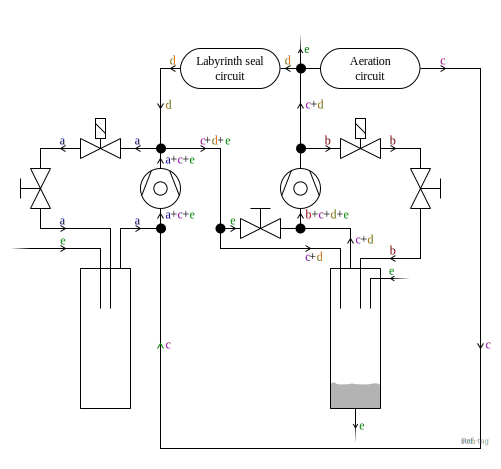
\includegraphics[width=\linewidth]{awp-bypass-mf}}
      \\
      \subfloat[BWP simplified bypass circuit layout]
      {\label{fig:bwp-bypass-simple-layout}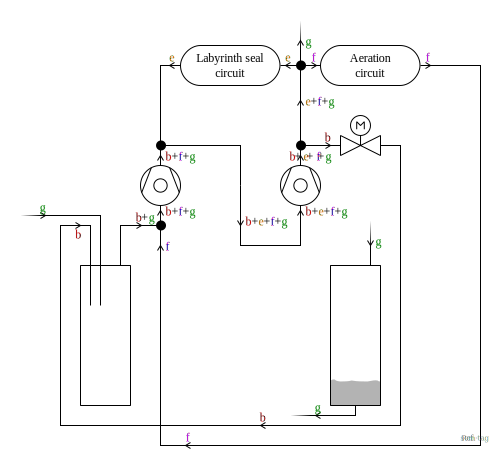
\includegraphics[width=\linewidth]{bwp-bypass-mf}}
    \end{flushright}
  \end{minipage} \hfill
  \begin{minipage}[l]{0.48\linewidth}
    \begin{flushleft}
      \subfloat[Bypass circuits characteristics in compressor maps]
      {\label{fig:bypass-in-maps}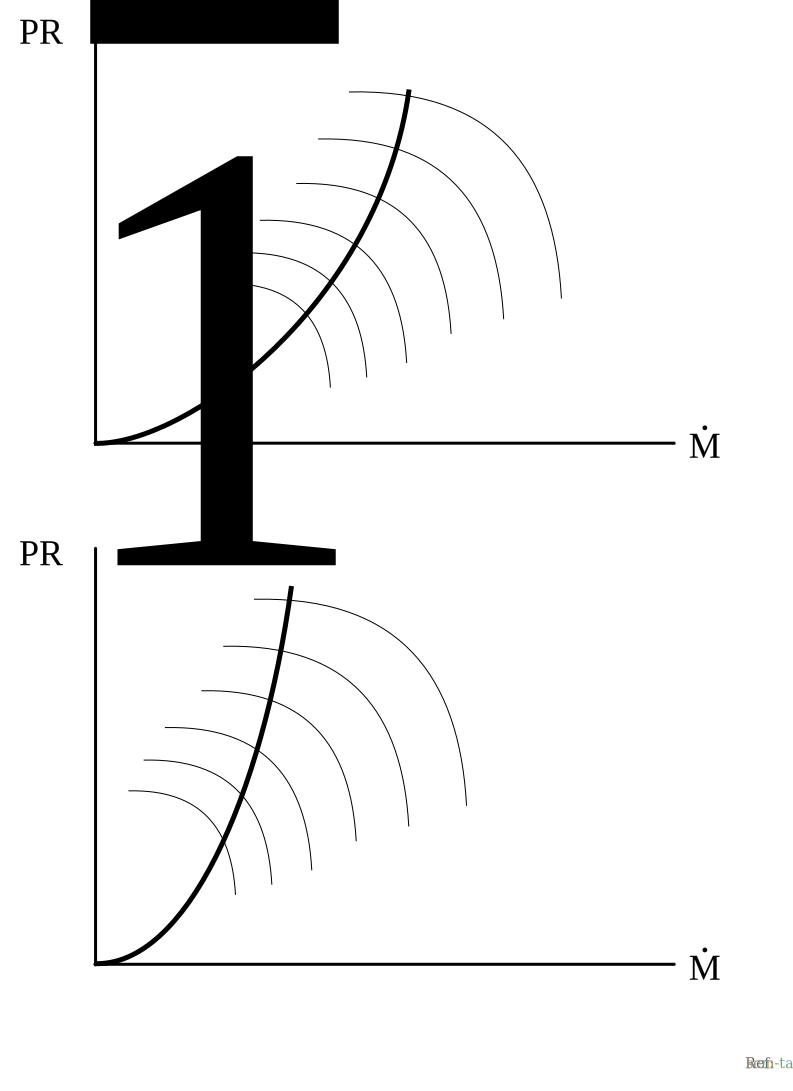
\includegraphics[width=\linewidth]{bypass-in-maps}}
    \end{flushleft}
  \end{minipage}
  \caption[Compressors bypass systems in the AWP and the
  BWP]{Compressors bypass systems in the AWP and the BWP. Those
    schematics are simplified layouts. The complete layouts are
    available in \cref{fig:awp-layout-model-numbers,fig:bwp-layout}.}
  \label{fig:bypass-schematics}
\end{figure}

\subsection{Motor cooling circuit}
\label{sec:bwp-motor-cooling}

The motor cooling circuit in the \BWP{} takes in account the motor
cooling issue encountered with the \AWP{} and detailed in
\cpref{sec:awp-issue-motor-cooling}. The motor cooling strategy in the
\BWP{} is based on a flow-boiling heat exchange while the strategy in
the \AWP{} is a pool-boiling strategy. Pool boiling is easier to
control as a simple liquid level management would be enough to ensure
the proper cooling down of the motor. As lubricant pollution is
encountered in the heat pump circuits\footnotep{This motor cooling
  issue is detailed in \cpref{sec:awp-issue-oil+corrosion}.}, flow
boiling was a better technical solution in polluted
circuits\footnotep{Details about the design and layout of the \BWP{}
  motor cooling circuit are given in
  \cpref{sec:bwp-motor-cooling-details}.}. The compression unit inlets
and outlets could be closed with ball valves, in order to be able to
remove the unit from the circuit without recovering the refrigerant
from the installation. The layout of the motor cooling circuit can be
observed in \cref{fig:bwp-layout}. The circuit is the component \#7.

\subsection{Gas bearings aeration circuit}
\label{sec:bwp-aeration}

The \BWP{} gas bearings circuit\footnotep{Further details about the
  BWP gas bearings aeration circuit can be found in
  \cpref{sec:bwp-aeration-details}.}  is similar to the \AWP{}, but
has the following main differences:

\begin{itemize}
\item The topology of the circuit is more vertical than in the \AWP{},
  and the pipes are longer. As a result, the pressure drop in the
  pipes is higher, and the chances of gas condensation in the pipes
  are also higher. However, the risk of condensation is decreased by
  the fact that the BWP is kept at room temperature, while the AWP was
  in the climate chamber, and was consequently at the environment
  temperature.
\item There are two 0.5\si{\micro\meter}-filters (one per circuit
  branch). Consequently the pressure drop created by the filtration
  process is lower.
\end{itemize}

The layout of the gas bearings aeration circuit can be observed in
\cref{fig:bwp-layout}. The circuit is made of the components \#21,
\#22, \#26, and of the pipe connecting component \#12 to component
\#19. The new layout was expected to solve the issue detailed in
\cpref{sec:awp-P-balance}. Unfortunately, the data collected and the
test performed did not allow to confirm the solving of the issue
with the new system, as the compression unit broke before a proper
stop sequence could be studied. Consequently, further tests with new
compression units and the next version of the experimental setup need
to be performed with the improved bypass circuit in order to document
the new system and its results.

\section{Modeling}
\label{sec:bwp-model}

The model proposed is based on the areas or physical elements of
interest in the \BWP{}. \Cref{fig:bwp-layout} presents the \BWP{}
layout and \cref{fig:bwp-maillefer-break-model} presents the model
itself. The set of equations deduced from analysis of the model in
\cref{fig:bwp-maillefer-break-model} is detailed in
\cref{chap:bwp-eqn}. Following the procedure described in
\cpref{sec:methodo-models}, the model is built with 27 components; 10
of them describe the compression unit itself.

\begin{figure}
  \centering
  \includegraphics[width=0.95\textwidth]{bwp-maillefer-exp-analysis-model-break}
  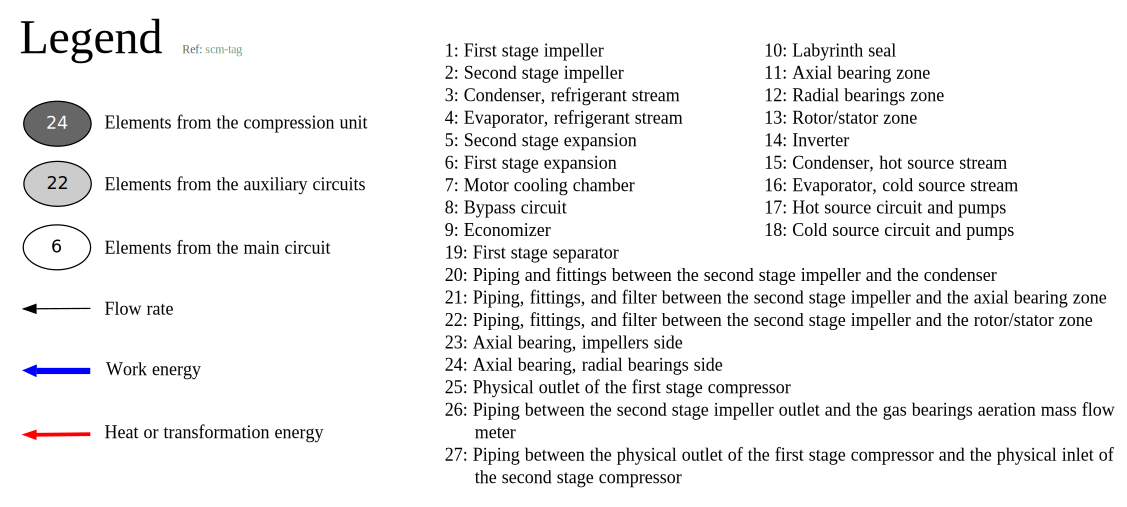
\includegraphics[width=0.95\textwidth]{bwp-maillefer-exp-analysis-model-break-legend}
  \caption[Modeling of the BWP in bypass mode]
  {Modeling of the BWP in bypass mode. The bypass mode implies that
    the two compression stages are connected in series.}
  \label{fig:bwp-maillefer-break-model}
\end{figure}

\section{BWP results and observations}
\label{sec:bwp-perfs}

The compression unit failed after 25 minutes of experiment, while an
\OP{} B8.0/W11.0 was being stabilized. The \OP{} in question was not
really a conventional \OP{}, as the compression unit was still
bypassed. The experimenter was stabilizing the conditions before
closing the bypass circuit furthermore. Using the model proposed in
\cref{sec:bwp-model}, the amount of the flow being bypassed could be
computed. At the time when the compression unit broke, 61\% of the
flow was being bypassed\footnotep{Ratio of $\dotM{8}{19}$ over
  $\dotM{1}{25}$. The values of those mass flow rate are available in
  \cpref{tab:bwp-B8.0/W11.0-mf}.}, which explains the high level of
superheat observed at the outlet of the first stage separator
(component \#19).

Using the model, the mass flow rates and the energy rates between the
components of the prototype could be computed. They are detailed in
\cref{tab:bwp-B8.0/W11.0-mf,tab:B8.0/W11.0-energy-flows}\footnotep{The
  thermodynamic points, the performance indicators, and the graphs of
  some key values right before the break are available in
  \cpref{sec:bwp-exp-details-B8.0/W11.0}.}. Observing the data
collected from the experiment or determined with the model leads to
the following general observations:

\begin{itemize}
\item Changing the gas bearings aeration circuit inlets/outlets
  configuration used for the \AWP{} to the proper configuration,
  applied in the \BWP{}, seems to change the temperature behavior in
  the compression unit, as it can be observed in
  \cref{fig:bwp-B8.0/W11.0-Ts}, compared with the behavior observed
  with the closest \AWP{} \OP, represented in
  \cref{fig:awp-A-0.5/W20.7-Ts}, where the temperature was increasing
  a lot less in the aeration circuit.
\item The motor cooling flow was too high. This was done on purpose,
  in order for the experimenter to be able not to worry about the
  cooling of the motor during the start-up phase of the
  experiment. The compression unit internal temperature was monitored
  with a PT100 inside the compression unit. The PT100 was located on a
  metal part surrounding the radial bearings cavity. At the time of
  the break, the temperature was of about
  35\si{\degreeCelsius}\footnotep{This temperature was screened on an
    independent device and was not recorded by the data acquisition
    system.}.
\item \Cref{tab:bwp-B8.0/W11.0-mf} shows that there was approximately
  no flow in the labyrinth seal\footnotep{Component \#10.}, and that
  this flow was almost adiabatic, which seems to indicate that the
  shaft was not at a high temperature at the time and that the
  impellers were at a temperature close to the second stage gas outlet
  temperature.
\item The gas in the bypass circuit (component \#8) was not increasing
  its temperature too much despite the relatively long period of
  bypassing involved\footnotep{The bypass circuit has been partially
    opened for the whole time of the experiment: 25 minutes. Despite
    this, the gas temperatures were reasonable, as it can be observed
    in \cpref{tab:B8.0/W11.0-PThs}.}.
\end{itemize}

\Cref{tab:key-values-comp-awp-bwp,fig:bwp-B8.0/W11.0-A-0.5/W20.7-diagrams}
allow to compare the situation between the lower \OP{} from the \AWP{}
, the \OP{} A-0.5/W20.7, and the \OP{} from the \BWP{}, to some extend
and on specific topics\footnotep{Original values can be retrieved from
  \cpref{tab:A-0.5/W20.7-PThs}, \cpref{tab:A-0.5/W20.7-energy-flows},
  \cpref{tab:B8.0/W11.0-PThs}, and
  \cref{tab:B8.0/W11.0-energy-flows}.}. The temperature values from
\cref{tab:key-values-comp-awp-bwp} illustrate that the compression
unit thermal behavior is very different in the \BWP{} and in the
\AWP{}. The two \OP{} can not be compared easily as the following
important differences can be observed:

\begin{itemize}
\item The heat energy rate from the motor to the shaft is 5 times
  higher in the \AWP{} \OP{} than in the \BWP{} \OP{}.
\item The \BWP{} \OP{} is recorded at a rotor speed of 110 krpm while
  the \AWP{} \OP{} is recorded at a rotor speed of 130 krpm.
\end{itemize}

Those differences do not formally allow the author to compare the
thermal behavior of the two units. Indeed, the gas inlet temperatures
and rotor speeds are comparable but the heat energy rates from the
motor to the shaft are very different. Consequently the following
comparisons are trends that need to be evaluated with further
experiments, with new compression units in a next version of the
\BWP{}. If the \OP{} would be comparable, the following interesting
points would be interesting to stress:

\begin{itemize}
\item The maximum temperature, occurring in the \AWP{} compression unit
  in the axial bearing, occurs in the \BWP{} compression unit at the
  outlet of the gap between rotor and stator.
\item The maximum gas temperature in the \AWP{} is more than 7 times
  higher than in the \BWP{}. The gas temperature at the outlet of the
  axial bearing sides is only few degrees hotter in the \BWP{}
  compression unit while it is several tenths of degree hotter in the
  \AWP{} compression unit, even despite of the flows in the bearings
  that are in the same order of magnitude in the two experimental
  setups, as the inlet mass flow rate between the two experiments had
  been kept at the same value\footnotep{The mass flow rates in the
    \AWP{} A-0.5/W20.7 \OP{} are available in
    \cpref{tab:awp-A-0.5/W20.7-mf}, and the mass flow rates in the
    \BWP{} B8.0/W11.0 \OP{} are available in
    \cref{tab:bwp-B8.0/W11.0-mf}.}.
\item The temperature of the flow in the labyrinth seal of the \BWP{}
  compression unit is almost constant and is very close to the
  temperature hottest gas flowing in the impellers. This allows to
  think that the impellers temperature was close to
  \num{51}\si{\degreeCelsius} during the \BWP{} \OP{}, as the gas
  temperature reaches \num{51}\si{\degreeCelsius} at the seal outlet
  and as the flow in the labyrinth seal is very small. As stressed in
  \cpref{sec:awp-laby-hot-gas}, the temperature of the impellers in
  the \AWP{} were probably much higher.
\end{itemize}

\begin{table}[htbp]
  \footnotesize
  \centering
\begin{tabular}{lcccccccc}
  \toprule
  \multirow{2}{*}{OP and speed} &
  \multicolumn{2}{c}{Motor} &
  \multicolumn{3}{c}{Gas bearings aeration} &
  \multicolumn{2}{c}{Labyrinth seal}\\
  & $\dotQ{13}{12}$ / \si{\watt} &
  $T_{13,out}$ / \si{\degreeCelsius} & In \#1 / \si{\degreeCelsius} &
  In \#2 / \si{\degreeCelsius} & Out / \si{\degreeCelsius} &
  In / \si{\degreeCelsius} & Out / \si{\degreeCelsius}\\
  \midrule
  B8.0/W11.0, 110 krpm & $\num{11.685} \pm \num{0.003}$ & $\num{17} \pm \num{19}$ & $\pmb{\num{7.90} \pm \num{0.01}}$ & $\pmb{\num{7.98} \pm \num{0.01}}$ & $\pmb{\num{18.95} \pm \num{0.01}}$ & $\num{50.7} \pm \num{0.2}$ & $\num{51} \pm \num{8}$ \\
  A-0.5/W20.7, 130 krpm & $\num{53.060} \pm \num{0.009}$ & $\num{14} \pm \num{23}$ & $\pmb{\num{6.271} \pm \num{0.007}}$ & $\pmb{\num{6.271} \pm \num{0.007}}$ & $\num{123} \pm \num{57}$ & $\num{32} \pm \num{2}$ & $\num{46} \pm \num{21}$ \\
  \bottomrule
\end{tabular}
\caption[Key values for the comparison of the AWP and the BWP gas bearings aeration circuits, regarding thermal management]{Key values for the comparison of the AWP and the BWP gas bearings aeration circuits, regarding thermal management. The values are rounded to the unit.}
\label{tab:key-values-comp-awp-bwp}
\end{table}

\begin{figure}[htbp]
  \centering
  \subfloat[B8.0/W11.0 -- Refrigeration diagram]
  {\label{fig:bwp-B8.0/W11.0-Ph}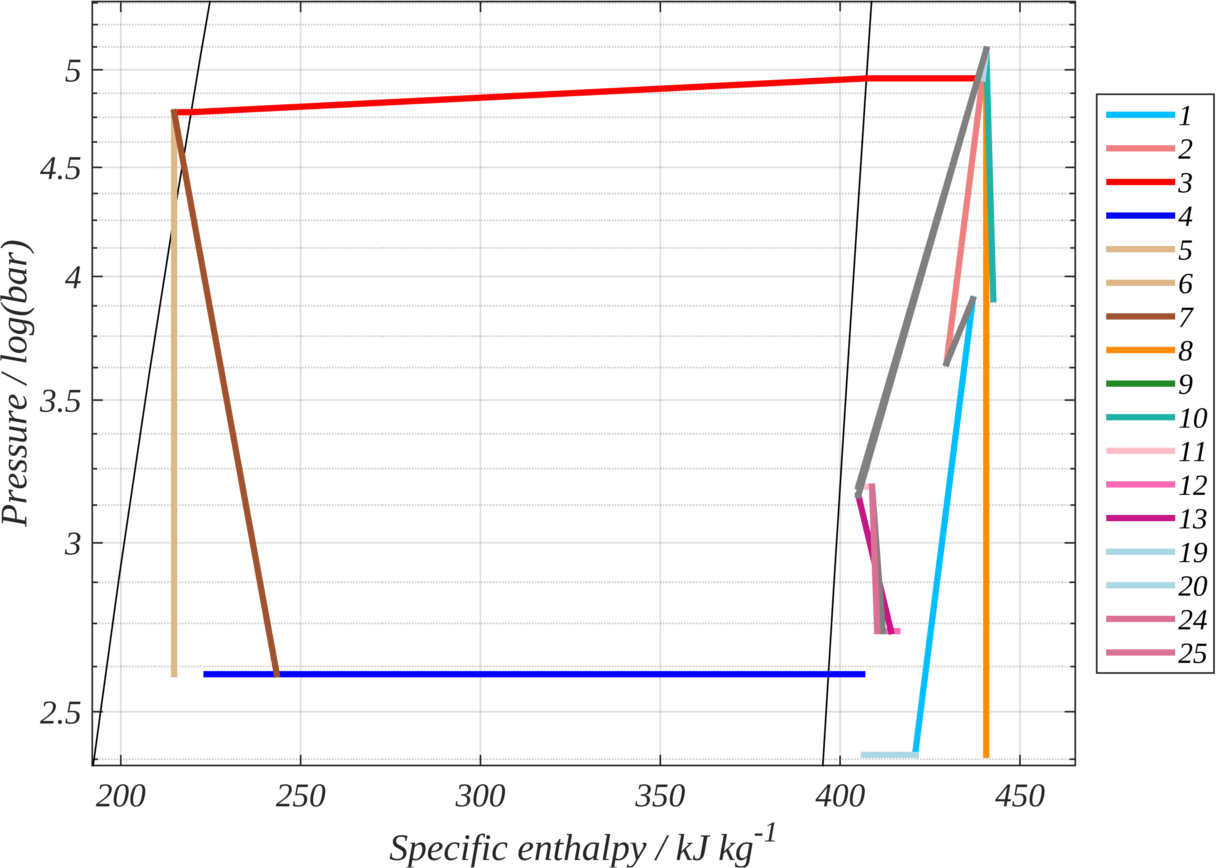
\includegraphics[height=50mm]{bwp-Ph-break}}
  \hspace{1em}
  \subfloat[B8.0/W11.0 -- Entropic diagram]
  {\label{fig:bwp-B8.0/W11.0-Ts}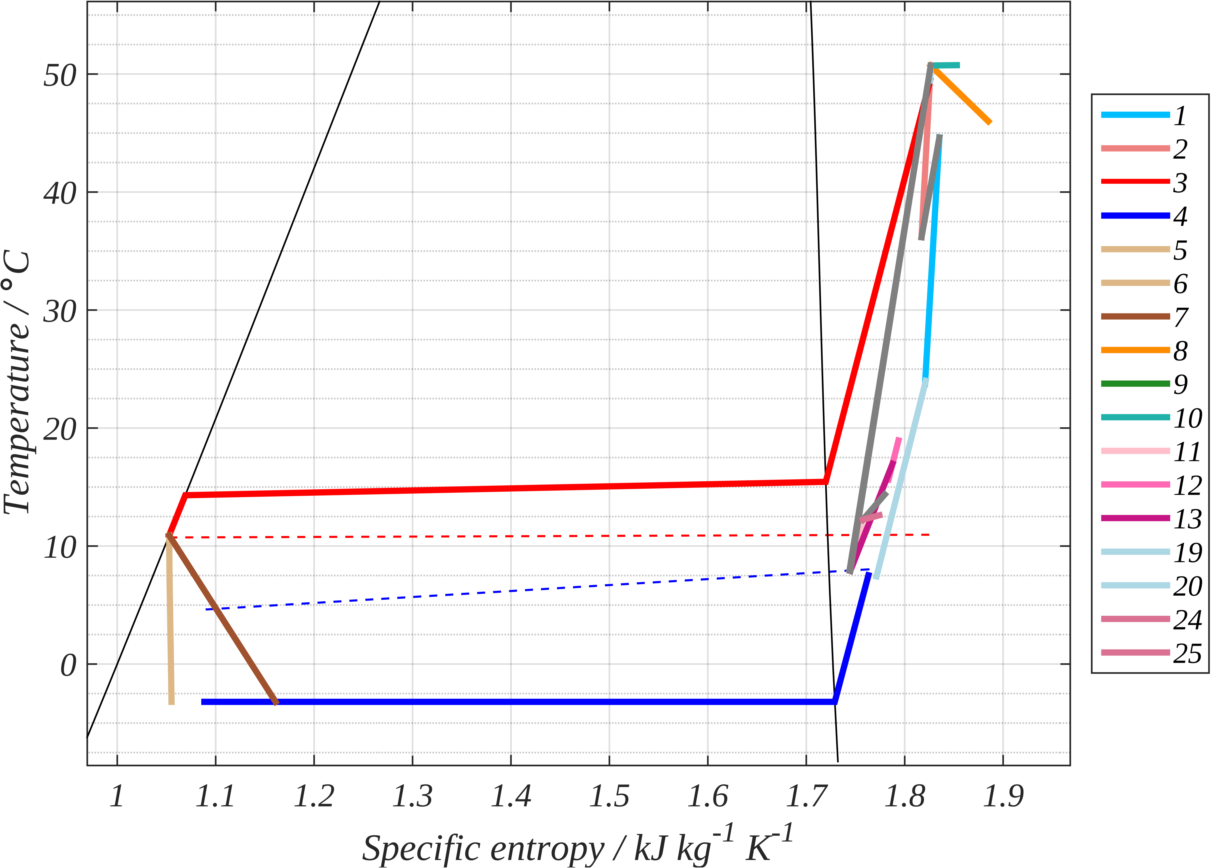
\includegraphics[height=50mm]{bwp-Ts-break}}
  \\
  \subfloat[A-0.5/W20.7 -- Refrigeration diagram]
  {\label{fig:awp-A-0.5/W20.7-Ph}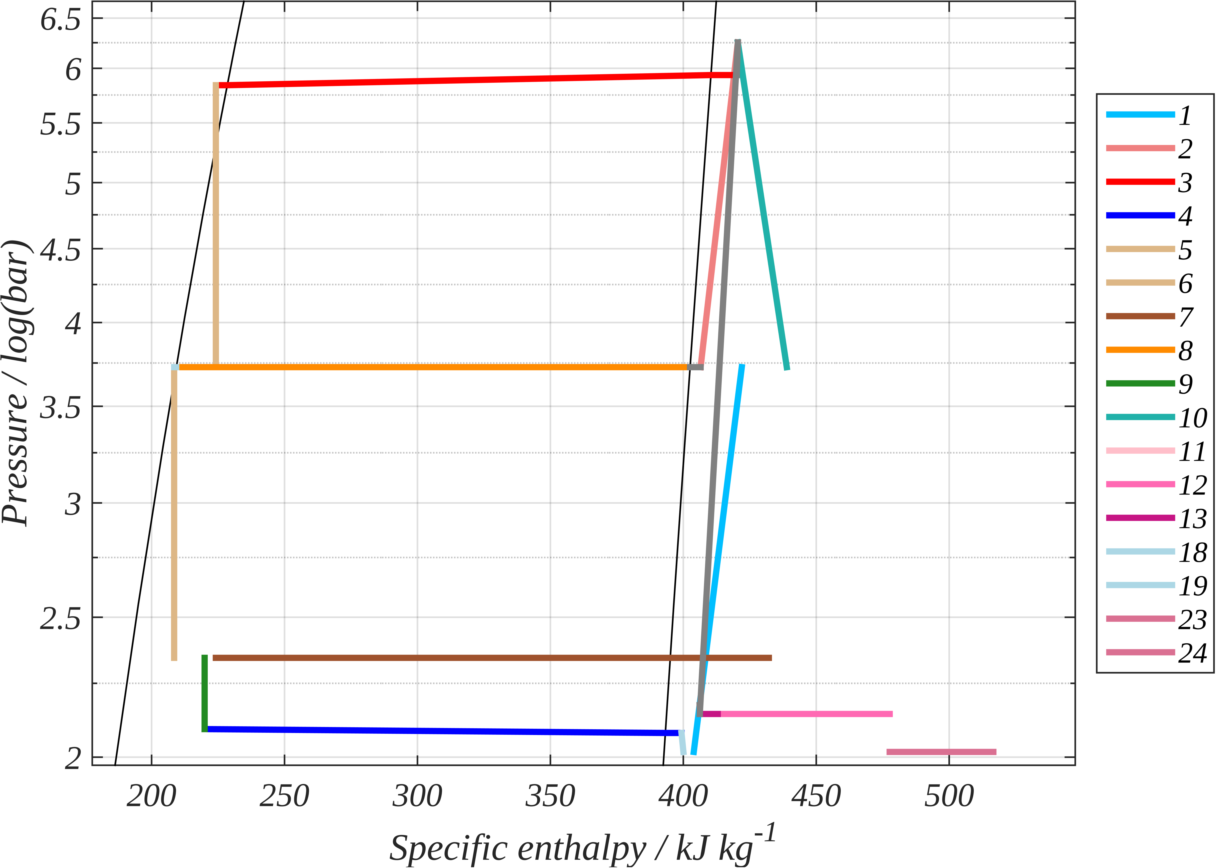
\includegraphics[height=50mm]{awp-Ph-20120531-093353-093653}}
  \hspace{1em}
  \subfloat[A-0.5/W20.7 -- Entropic diagram]
  {\label{fig:awp-A-0.5/W20.7-Ts}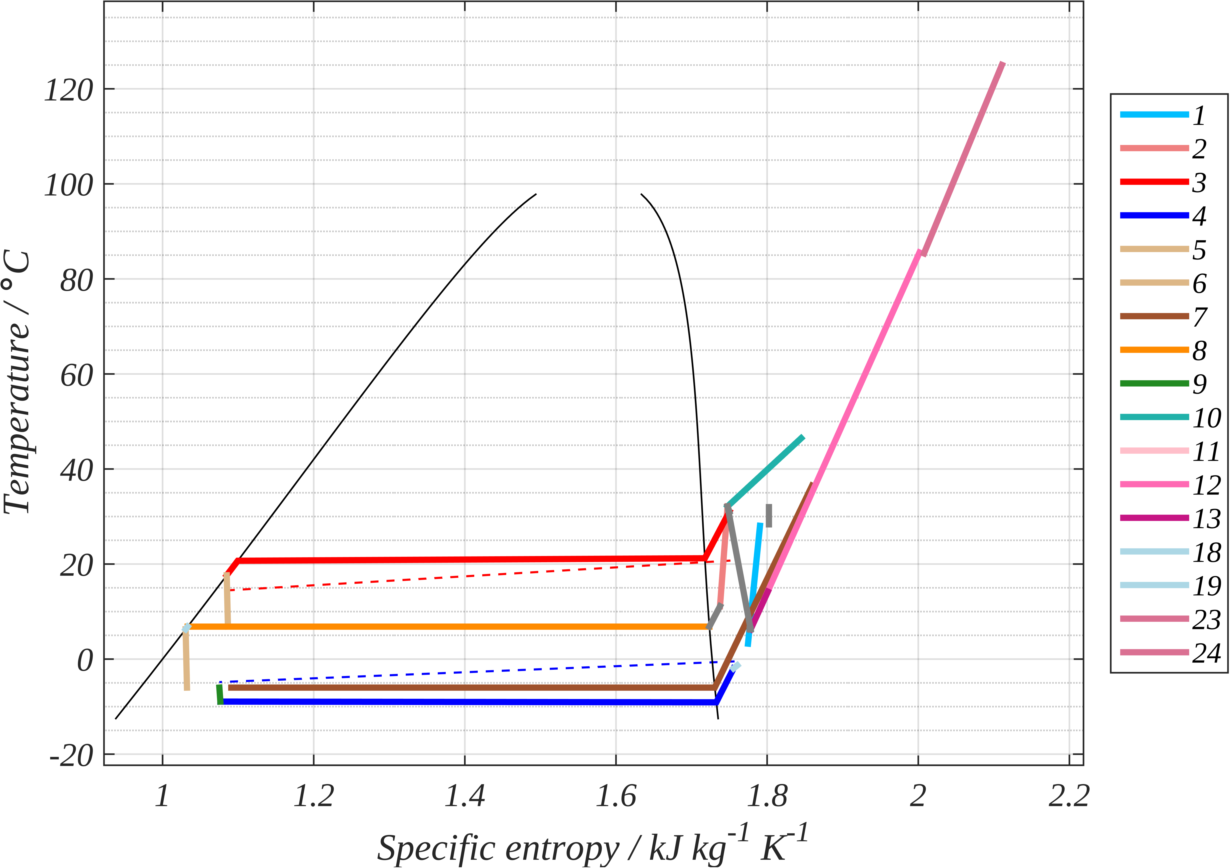
\includegraphics[height=50mm]{awp-Ts-20120531-093353-093653}}
  \caption[Thermodynamic diagrams of the BWP OP and of its closer AWP
  OP]{Thermodynamic diagrams of the BWP OP and of its closer AWP
    OP. Those diagrams are presented together in order to give
    comparison opportunities between the two prototypes behavior.}
  \label{fig:bwp-B8.0/W11.0-A-0.5/W20.7-diagrams}
\end{figure}

\begin{table}[htbp]
    \footnotesize
    \begin{center}
      \begin{tabular}{llllll}
\toprule
Name & Value / \si{\gram\per\second} & Name & Value / \si{\gram\per\second} & Name & Value / \si{\gram\per\second} \\
\midrule
$\dot{M}_{1 \rightarrow 25}$ & $ \num{29.2} \pm \num{0.3} $ & $\dot{M}_{2 \rightarrow 8}$ & $ \num{17.8} \pm \num{0.2} $ & $\dot{M}_{2 \rightarrow 10}$ & $ \num{1.88275618e-06} \pm \num{2e-06} $ \\
$\dot{M}_{2 \rightarrow 20}$ & $ \num{10.1} \pm \num{0.2} $ & $\dot{M}_{2 \rightarrow 26}$ & $\pmb{ \num{1.20} \pm \num{1.20} }$ & $\dot{M}_{3 \rightarrow 5}$ & $\pmb{ \num{6.94} \pm \num{6.94} }$ \\
$\dot{M}_{3 \rightarrow 7}$ & $\pmb{ \num{3.20} \pm \num{3.20} }$ & $\dot{M}_{4 \rightarrow 19}$ & $ \num{10.1} \pm \num{0.2} $ & $\dot{M}_{5 \rightarrow 9}$ & $ \num{6.94} \pm \num{6.94} $ \\
$\dot{M}_{6 \rightarrow 4}$ & $ \num{6.94} \pm \num{6.94} $ & $\dot{M}_{7 \rightarrow 4}$ & $ \num{3.2} \pm \num{3.2} $ & $\dot{M}_{8 \rightarrow 19}$ & $ \num{17.8} \pm \num{0.2} $ \\
$\dot{M}_{9 \rightarrow 6}$ & $\pmb{ \num{6.94} \pm \num{6.94} }$ & $\dot{M}_{10 \rightarrow 25}$ & $ \num{1.88275618e-06} \pm \num{2e-06} $ & $\dot{M}_{11 \rightarrow 23}$ & $ \num{0.71} \pm \num{0.71} $ \\
$\dot{M}_{11 \rightarrow 24}$ & $ \num{0.151} \pm \num{0.151} $ & $\dot{M}_{12 \rightarrow 19}$ & $ \num{0.49} \pm \num{0.49} $ & $\dot{M}_{13 \rightarrow 12}$ & $ \num{0.34} \pm \num{0.34} $ \\
$\dot{M}_{19 \rightarrow 1}$ & $ \num{28.5} \pm \num{0.3} $ & $\dot{M}_{20 \rightarrow 3}$ & $ \num{10.14} \pm \num{10.14} $ & $\dot{M}_{21 \rightarrow 13}$ & $ \num{0.34} \pm \num{0.34} $ \\
$\dot{M}_{22 \rightarrow 11}$ & $ \num{0.86} \pm \num{0.86} $ & $\dot{M}_{23 \rightarrow 1}$ & $ \num{0.71} \pm \num{0.71} $ & $\dot{M}_{24 \rightarrow 12}$ & $ \num{0.151} \pm \num{0.151} $ \\
$\dot{M}_{25 \rightarrow 27}$ & $ \num{29.2} \pm \num{0.4} $ & $\dot{M}_{26 \rightarrow 21}$ & $ \num{0.34} \pm \num{0.34} $ & $\dot{M}_{26 \rightarrow 22}$ & $ \num{0.86} \pm \num{0.86} $ \\
$\dot{M}_{27 \rightarrow 2}$ & $ \num{29.2} \pm \num{0.4} $ \\
\bottomrule
\end{tabular}

    \end{center}
    \caption{B8.0/W11.0 -- Mass flow rates between the components}
    \label{tab:bwp-B8.0/W11.0-mf}
\end{table}

\begin{table}[htbp]
    \footnotesize
    \begin{center}
    \begin{tabular}{llll}
\toprule
Name & Value / $W$ & Name & Value / $W$ \\
\midrule
$\dot{E}_{1 \rightarrow 2}$ & $ \num{322} \pm \num{5} $ & $\dot{E}_{11 \rightarrow 1}$ & $ \num{791.8} \pm \num{0.2} $ \\
$\dot{E}_{12 \rightarrow 11}$ & $ \num{824.9} \pm \num{0.2} $ & $\dot{E}_{13 \rightarrow 12}$ & $ \num{844.3} \pm \num{0.2} $ \\
$\dot{E}_{14 \rightarrow 13}$ & $ \num{950.4} \pm \num{0.2} $ & $\dot{E}_{cp1}$ & $ \num{469} \pm \num{5} $ \\
$\dot{E}_{cp2}$ & $ \num{322} \pm \num{5} $ & $\dot{E}_{el \rightarrow 14}$ & $\pmb{ \num{1118.1} \pm \num{0.2} }$ \\
$\dot{Y}_{1 \rightarrow 2}$ & $ \num{2.1718939e-05} \pm \num{1e-07} $ & $\dot{Y}_{2 \rightarrow 10}$ & $ \num{3.71518884e-06} \pm \num{2e-08} $ \\
$\dot{Y}_{3 \rightarrow 15}$ & $ \num{2280} \pm \num{25} $ & $\dot{Y}_{11 \rightarrow 1}$ & $ \num{59.3} \pm \num{0.3} $ \\
$\dot{Y}_{11 \rightarrow 23}$ & $ \num{6.315950126e-07} \pm \num{3e-09} $ & $\dot{Y}_{11 \rightarrow 24}$ & $ \num{0.216} \pm \num{0.001} $ \\
$\dot{Y}_{12 \rightarrow 11}$ & $ \num{29.6} \pm \num{0.3} $ & $\dot{Y}_{13 \rightarrow 7}$ & $ \num{91.31} \pm \num{0.02} $ \\
$\dot{Y}_{13 \rightarrow 12}$ & $ \num{11.685} \pm \num{0.002} $ & $\dot{Y}_{14 \rightarrow at}$ & $ \num{167.72} \pm \num{0.04} $ \\
$\dot{Y}_{16 \rightarrow 4}$ & $ \num{1849} \pm \num{53} $ & $\dot{Y}_{20 \rightarrow at}$ & $ \num{10} \pm \num{10} $ \\
$\dot{Y}_{21 \rightarrow at}$ & $ \num{12} \pm \num{9} $ & $\dot{Y}_{22 \rightarrow at}$ & $ \num{30} \pm \num{22} $ \\
$\dot{Y}_{27 \rightarrow at}$ & $ \num{214} \pm \num{189} $ & $\dot{Q}_{ax}$ & $ \num{33.1} \pm \num{0.3} $ \\
$\dot{Q}_{mo}$ & $ \num{106.12} \pm \num{0.02} $ & $\dot{Q}_{ra}$ & $ \num{19.4} \pm \num{0.3} $ \\
\bottomrule
\end{tabular}

  \end{center}
  \caption{B8.0/W11.0 -- Energy rates between the components}
  \label{tab:B8.0/W11.0-energy-flows}
\end{table}

\section{Additional issues}
\label{sec:bwp-issues}

\subsection{Getting enough power to explore the operation range}
\label{sec:bwp-issue-power}

The compression unit runs at really high speed and consequently needs
an inverter able to provide the needed electric power at the needed
frequency. Finding such an inverter in the current inverter market is
problematic, as high speed drive applications currently applies to
lower electric powers than the one requested for this
work\footnotep{The twin-stage compression unit requires an electric
  power of \num{6} \si{\kilo\watt} to be able to explore its whole
  operation range.}. Consequently, the development of such an inverter
showed up to be necessary and has been performed during an other
thesis work \citep{rod-2012a}. \citet[fig. 6.6, p.\,118]{rod-2012a} has
developed a prototype of inverter which could have been used to power
the compression unit. This prototype needs to be developed further to
become an industrial prototype, ready to used with the compression
units \citep[p.\,134]{rod-2012a}. The experiments have not been
performed with the inverter developed by \citep{rod-2012a}, as it was
still a device in development when the experiments were performed, and
the prototypes had to cope with the limits of industrial inverters
which were able to explore only partly the prototypes operation
domain. Even nowadays, the development and the industrialization of
such an inverter is a critical issue for the power and control of the
heat pumps equipped with such compression
units \citep[p.\,135]{rod-2012a}.

\subsection{Setting the intermediate pressure to a chosen value while being in bypass-mode}
\label{sec:bwp-bypass-mode-Pint-issue}

When being in bypass-mode, the two compression stages have the same
mass flow rate, as they are connected in series. If the flow is only
partially bypassed, the overall pressure ratio is imposed by the
temperature of the sources. As the compression unit rotor speed is a
fixed parameter at a given time, the pressure level between the two
compression stages is a consequence of the compressor maps and can not
be set to a chosen value, as it can be seen in
\cpref{fig:awp-control-ppe-2cp}, considering the same mass flow rate
for the two stages. To be able to close the bypass circuit completely
and to switch to normal-mode, the pressure level in the economizer has
to be kept equal to the pressure level between the compression
stages. If this is not done, the switch can occur nonetheless, but a
pressure shock wave is likely to occur. Because of the check valve at
the first compression stage outlet, the economizer pressure level can
not be below the first stage outlet pressure level, even while being
in bypass-mode. Consequently, the pressure level in the economizer is
necessarily equal (or, eventually, slightly lower\footnotep{Because of
  the pressure drop in the pipes, the pressure level at the inlet of
  the second compression stage can be slightly lower than the pressure
  level at the gas outlet of the economizer.}) or higher than the
pressure level at the second stage inlet. Consequently, the shock wave
will be directed from the second compression stage to the economizer
and will occur when the valve between components \#9 and \#2
opens. This counter flow shock wave can create instabilities in the
flow inside the second stage impeller, damaging blades, or even
produce a compression unit failure. In order to prevent such an event
to occur, the pressure level in the economizer during bypass-mode needs
to be kept at the pressure level of the second compression stage. This
also ensure that no flow comes in the economizer from the first
compression stage.  The pressure level in the economizer while being
in bypass-mode is influenced only by the settings of the two expansion
valves (considering that the economizer is properly insulated from the
environment and consequently adiabatic). As the role of the first
stage expansion valve is to maintain a superheat value at the
evaporator outlet, even during bypass-mode, the pressure level is
maintained at the second compression stage inlet pressure level by the
second stage expansion valve only. If the pressure level in the
economizer decreases, the valve opens, and if it increases, the valve
closes. If there is no more liquid in the economizer, the second stage
expansion valve closes to a minimal value, in order to let the
pressure level in the condenser increase (this is the second expansion
valve starting-mode explained in \cpref{sec:awp-issue-control-indus}).

\subsection{Pumping down of the evaporator}
\label{sec:pump-down-ev}

In a heat pump circuit, it might happen situations where all the
liquid refrigerant charge is located in the evaporator. This is the
case, for example, when you fill in the refrigerant charge in gas
phase being condenser at the coldest location of the circuit (the
evaporator). It can also be the case if the expansion valves are not
fully closed when the installation is shut down and if some time
passes between the shutdown and the next start up (in case of power
failure, for instance). With the bypass system used in the
\AWP{}\footnotep{The layout of this bypass system can be seen in
  \cpref{fig:awp-bypass-simple-layout} and
  \cpref{fig:awp-layout-model-numbers}.}, it is almost impossible to
pump down the liquid in the evaporator using the compression unit and
the condenser, as it can be seen in
\cref{fig:bwp-pumpdown-ev}. Indeed, as the bypass circuits are either
closed or opened (no in-between position), and as there is no way to
create a significant pressure difference in the heat pump main circuit
without closing one of the bypass circuits (which would most likely
results in moving the compression stages into the surge domain), all
the liquid stays in the evaporator. The only way that could be found
during the experimental campaign was to decrease the temperature at
the condenser, allowing to close the second stage bypass circuit. With
the second stage bypass circuit being closed, the pressure in the
condenser increases and the flows starts to condense. Refrigerant is
being transferred from the evaporator to the condenser. Some liquid
finally arrives in the economizer and the cycle can be started.

\begin{figure}
  \centering
  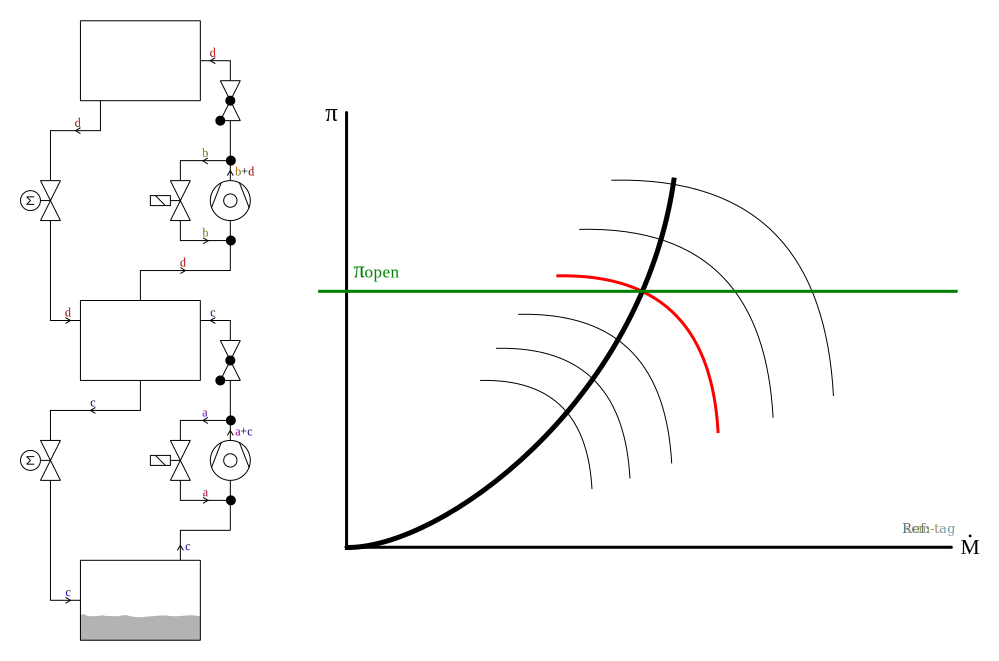
\includegraphics[width=\textwidth]{bwp-pump-down}
  \caption[Simplified layout in an evaporator pump down situation]
  {When a pump down of the evaporator is needed, most of the liquid
    refrigerant is in the evaporator and as there are almost no flow
    rate through the expansion valves (which are sized to be fed with
    liquid, not with gas), bypass circuits need to be opened to avoid
    the surge domain. If the rotor speed is high enough, the pressure
    ratio reached allows to move the check valves and some flow enters
    the main heat pump circuit. Unfortunately, in order to increase
    the pressure ratio in the condenser (which would allow the
    condensation process to occur), the expansion valve needs to
    close, reducing further the flow. The flow is then very small, and
    almost no liquid is transferred from the evaporator to the
    condenser. Meanwhile, there is no flow in the motor cooling
    circuit as there is no liquid in the condenser, and the motor
    temperature increases. It increases even faster as the rotor speed
    is high. If a bypass circuit is closed, the compression stage not
    being bypassed enters the surge domain, as there is not enough
    mass flow circulating in the heat pump circuit and a too big
    pressure ratio. Consequently, if the temperature between the
    sources is not reduced, there is no way to start the heat pump in
    this situation. The new bypass system is expected to solve this
    situation.}
  \label{fig:bwp-pumpdown-ev}
\end{figure}

With the new \BWP{} bypass system, the flow of both compressors is
bypassed together and pumping down the evaporator should not be a
problem. Indeed, the bypass-mode transforms the twin-stage circuit in
a single-stage circuit with the ability to bypass a chosen share of
the flow, and consequently, it should solve the issue described above.

\subsection{Keeping the loop clean}
\label{sec:awp-issue-oil+corrosion}

The prototypes tested use refrigerant with no lubricant. If there is
lubricant in the refrigerant, it causes circuit pollution problems. If
the pollution is not miscible in the refrigerant, it soaks the heat
exchangers surfaces, which is likely to decrease there heat transfer
efficiency \citep{BandarraFilho-Thome-2009a}. If it is miscible, it
decreases the heat power capacity of the heat exchangers. Moreover,
the lubricant is likely to enter the gas bearings and to fill their
grooves, causing their failure and a crash of the compression unit. If
grooves are polluted with oil, the probable consequence is a
displacement of the shaft in the bearing gap, which is likely to cause
a contact between the shaft surface and a fixed part. Touching a fixed
surface at that speed is likely to create torsion forces far beyond
the resistance of the shaft and to break it. Where the shaft touches a
fixed part, the energy released locally is high enough to weld the
surfaces together, damaging the unit massively. Such failure are
critical events and usually imply the full replacement of the
compression unit. Consequently, introducing clean refrigerant in the
heat pump circuits is very important. However, industrial refrigerant
cylinders often contain a small amount of synthetic lubricant
oil. This lubricant oil is likely to pollute the prototype circuits if
filled up with liquid refrigerant\footnotep{Liquid refrigerant can be
  filled in an installation either with a supply bottle put
  up-side-down, or with a recovery cylinder, using the liquid valve,
  which directly get liquid refrigerant from the bottom of the
  cylinder. The recovery cylinders may also contain mineral oil,
  leaked from the vacuum pump, for instance. This oil will be also
  transferred to the heat pump circuits, if they are filled up with
  liquid refrigerant.}. If the prototypes are filled up with gas being
condensed in one of the heat exchangers of the prototypes, some oil
can also pollute the circuits, as the gas velocity is high enough to
drag an oil film, flowing from the cylinder to the circuits of the
prototypes, on the wall of the tubes. In order to prevent oil flowing
from the cylinders to the circuits of the prototypes, gas velocity
need to be lower than a specific value which can be computed for each
specific design case \citep{kesim-ileri-2000a,Guo-Shen-2011a}. As
those design rules were not applied during the design of the heat pump
prototypes, lubricant oil could be observed flowing slowly from the
inlet of the first stage separator, at the top of the upper flange, to
the outlet, also located at the top of the upper flange, flowing on
the flange surface. The issue has been solved by adding a pipe and a
deflector, inside the separator, in order to make the way from the
inlet to the outlet less straightforward for the oil. The oil
pollution problem has been solved by decreasing dramatically the speed
of the filling up, doing it only with a low velocity, in gas phase. It
is important to note that a polluted installation is very difficult to
clean up, once it has been polluted. The synthetic lubricant oils have
low viscosity and surface tension, so they fill every possible
interstice. Consequently, every O-ring cavity, every welding, every
scratch, every groove or heat exchanger improved surface is polluted
and very difficult to clean up. The problem exists also with the
\AWP{} but extra care and protective behavior being applied from the
start helped to prevent a too high amount of oil pollution in the
circuits.

\begin{figure}
  \centering
  \begin{minipage}[r]{.49\linewidth}
    \begin{flushright}
      \subfloat[Lubricant droplets deposit]{\label{fig:bwp-oil-1}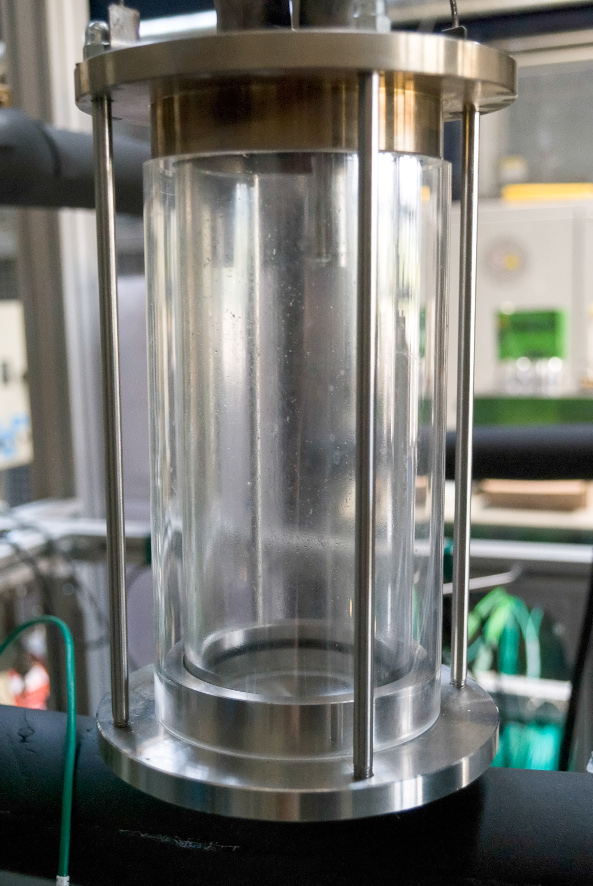
\includegraphics[height=10cm]{20110713T141014-1548d}}
    \end{flushright}
  \end{minipage} \hfill
  \begin{minipage}[l]{.49\linewidth}
    \begin{flushleft}
      \subfloat[Liquid lubricant]{\label{fig:bwp-oil-2}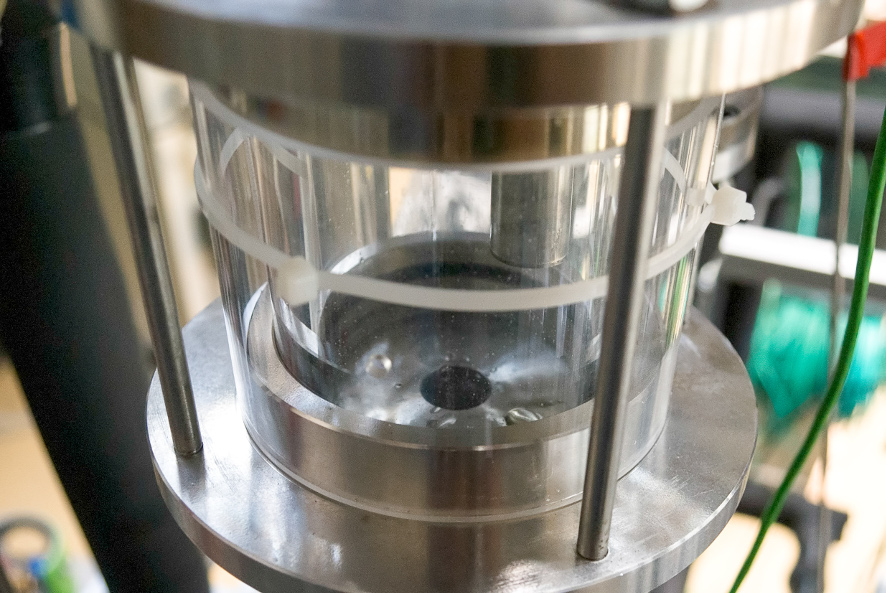
\includegraphics[width=6.45cm]{20110713T134430-1526d}} \\
      \subfloat[Lubricant and dusts]{\label{fig:bwp-oil-3}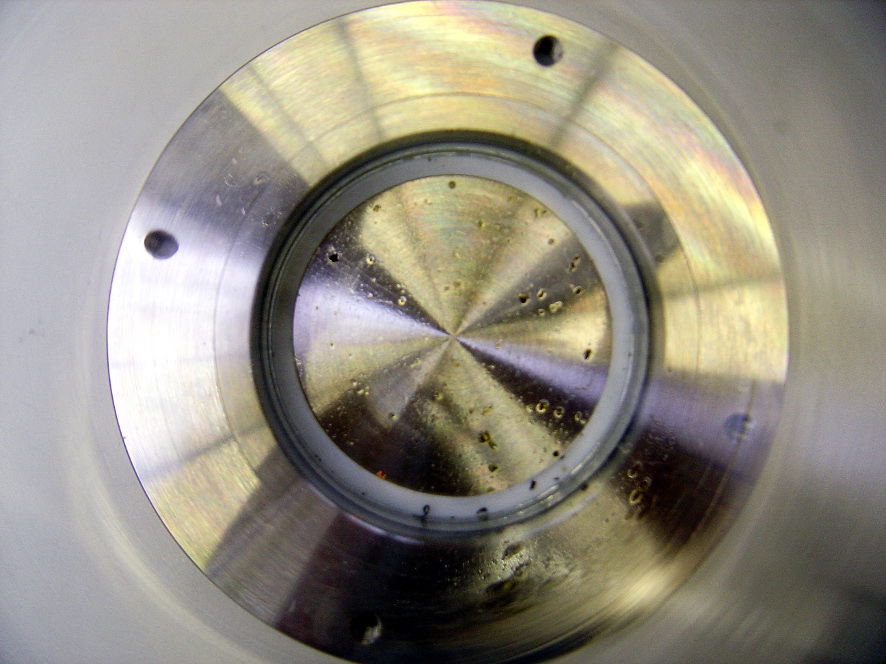
\includegraphics[width=6.45cm]{DSC00385}}
    \end{flushleft}
  \end{minipage}
  \caption{Lubricant pollution in the BWP}
  \label{fig:bwp-oil-pollution}
\end{figure}

Evaporators act as oil separation devices and tend to collect a good
share of the lubricant oil in the heat pumps circuits. In the \AWP{},
the motor cooling chamber and the evaporator play such a role. In the
\BWP{}, only the evaporator plays such a role, since the refrigerant
flows in the \BWP{} motor cooling chamber from top to bottom,
vertically, towards the evaporator. If the superheat value becomes too
low at the evaporator outlet, refrigerant and oil might flow in the
first stage separator, as illustrated in
\cpref{fig:bwp-oil-pollution}. Synthetic oil is miscible in liquid
R134a and will come with liquid refrigerant more or less
proportionally. Mineral oil, which comes from polluting elements in
the recovery cylinders, and from the vacuum pumps, stays on top of the
refrigerant liquid level. When some liquid comes from the evaporator,
the first amounts are heavily charged with mineral oil, if any is
present in the heat pump circuits. Oil reflux from the vacuum pumps is
something well known in the vacuum industry. Usually, this lubricant
oil is gasified and trapped with a catalyzer containing active
carbon. In the refrigeration industry, nothing is typically done
against those refluxes. Most of the refrigeration professionals even
ignore that such refluxes happen because they are not typically
problematic for the conventional refrigeration technologies, which use
lubrication, and consequently most of those professionals do not learn
the existence of this issue during their certification programs.

\FloatBarrier

\bibliographystyle{plainnat}
\bibliography{main}
\label{sec:bwp-refs}
